
\section{Market Sizing}\label{sec:markets}
% What to convey (Source: Pitch Perfect):
% What is our Market?
% What is the Market Size?
% What is the Market Trajectory

The market sizing parameters are listed in \cref{tab:market_size_params}. The description is given in \cref{subsec:market_introduction}.
\subsection{legend}
\begin{itemize}
	\item \textbf{bold} numbers are assumptions, used as model parameters (
	\item \textcolor{purple}{purple} words are cited datapoints used as model parameters.
	\item \textcolor{blue}{blue} numbers follow from the model parameters and assumptions.
\end{itemize}

\ifx\homepath\overleafhome
    % Overleaf compilation.
    \begin{longtable}{@{}cp{.7\textwidth}@{}}
    \caption{Cost Model Parameters in \euro (/hr or absolute, unlessspecified otherwise)}\label{tab:market_size_params}\\
    \toprule
    {\bfseries Parameter} & {\bfseries Value} \\ \midrule
    \endfirsthead
    \caption{Cost Model Parameters in \euro (/hr or absolute, unlessspecified otherwise) (continued)}\\
    \toprule
    \multicolumn{2}{l}{\scriptsize\emph{\ldots{} continued}}\\
    {\bfseries Parameter} & {\bfseries Value} \\ \midrule
    \endhead
    \multicolumn{2}{r}{\scriptsize\emph{to be continued\ldots}}\\
    \bottomrule
    \endfoot
    \bottomrule
    \endlastfoot
    nr simulations & 300.0\\
    profit dhl billion & 4.099999\\
    profit dhl & 4.100000e+09\\
    profit fedex billion & 1.29\\
    profit fedex & 1.290000e+09\\
    profit ups billion & 7.7\\
    profit ups & 7.700000e+09\\
    profit dhl fedex ups & 1.309000e+10\\
    sam factor & 0.003\\
    tam factor & 0.004\\
    logistics market share dhl fedex ups & 0.15\\
    logistics market share dhl fedex ups percentage & 15.0\\
    avg algo optimisation profit percentage & 0.1\\
    avg algo optimisation profit & 0.001\\
    TruCol cut on profit percentage & 1.0\\
    TruCol cut on profit & 0.01\\
\end{longtable}
 %\newpage
\else
    % Local compilation
    \begin{longtable}{@{}cp{.7\textwidth}@{}}
    \caption{Cost Model Parameters in \euro (/hr or absolute, unlessspecified otherwise)}\label{tab:market_size_params}\\
    \toprule
    {\bfseries Parameter} & {\bfseries Value} \\ \midrule
    \endfirsthead
    \caption{Cost Model Parameters in \euro (/hr or absolute, unlessspecified otherwise) (continued)}\\
    \toprule
    \multicolumn{2}{l}{\scriptsize\emph{\ldots{} continued}}\\
    {\bfseries Parameter} & {\bfseries Value} \\ \midrule
    \endhead
    \multicolumn{2}{r}{\scriptsize\emph{to be continued\ldots}}\\
    \bottomrule
    \endfoot
    \bottomrule
    \endlastfoot
    nr simulations & 300.0\\
    profit dhl billion & 4.099999\\
    profit dhl & 4.100000e+09\\
    profit fedex billion & 1.29\\
    profit fedex & 1.290000e+09\\
    profit ups billion & 7.7\\
    profit ups & 7.700000e+09\\
    profit dhl fedex ups & 1.309000e+10\\
    sam factor & 0.003\\
    tam factor & 0.004\\
    logistics market share dhl fedex ups & 0.15\\
    logistics market share dhl fedex ups percentage & 15.0\\
    avg algo optimisation profit percentage & 0.1\\
    avg algo optimisation profit & 0.001\\
    TruCol cut on profit percentage & 1.0\\
    TruCol cut on profit & 0.01\\
\end{longtable}
 %\newpage
\fi

\subsection{Introduction}\label{subsec:market_introduction}
To use the Top Down Model, \cref{subsec:total_addressable_market} describes the TAM in which the TruCol company will operate. To this end, \cref{subsubsec:tam_logistics} discusses the market size of the logistics market, and the profit within that market. Due to time-constraints and lack of data, some datapoints and assumptions of the logistics market are applied to other sectors such as the automated trading market and pharmaceutics market in \cref{subsubsec:additional_markets} to get some insight in their respective market sizes. Furthermore, \cref{subsubsec:emerging_markets} provides some qualitative insight in the potential future markets that are highly suited for the TruCol protocol. These emerging markets are accordingly expected to be relevant markets to address in the near future.

\subsection{Total Addressable Market}\label{subsec:total_addressable_market}
To compute the TAM, SAM and SOM, some form of market definition can be used. To this end, it is considered valuable to specify what the TruCol company does, where it adds value and how it does that. Furthermore, since these three aforementioned estimates pertain to a potential future, the potential, yet deemed feasible, activities of the TruCol company are included.
\\
The TruCol company provides advice and support to companies on how they can get the most out of the TruCol protocol. To understand this, the following assumptions are shared. Under these assumptions, one can conclude that an economically rational company would try to off-load as much of their required tasks into the TruCol protocol. This is because it would minimise their operational costs and/or improve algorithmic efficiency of their solutions.

\begin{itemize}
	\item \textbf{asu-0:} Solutions to tasks that are completed using the TruCol protocol are deterministically verifiable.
	\item \textbf{asu-1:} Solutions to tasks that are completed using the TruCol protocol are of sufficient quality.
	\item \textbf{asu-2:} Tasks that are completed using the TruCol protocol can be solved for the lowest cost price that is currently available in this world.
	\item \textbf{asu-3:} No personnel needs to be attracted, screened, hired nor fired for tasks that are completed using the TruCol protocol.
	\item \textbf{asu-4:} Companies can benefit from public particular solutions to their task specifications.
	\item \textbf{asu-5:} By sampling from a bigger talent pool (this world), the average performance of the solutions will be better than what is produced by the in-house talent pool, or, for equal solution performance, a faster rate of development can be obtained on average for an equal or lower price.
\end{itemize}



We help companies identify the tasks for which they can use the TruCol protocol, and we assist them in writing safe test specifications that are not easily hackable. This implies that under the given set of assumptions, the TAM for the TruCol protocol can be defined as the total costs that the companies (and consumers) in this world are willing to pay for assistance on using the TruCol protocol.

\subsubsection{TruCol Total Addressable Logistics Market}\label{subsubsec:tam_logistics}

This sub-sub section illustrates a rough method of estimating the logistics sub-segment of the TAM for the TruCol protocol. To do this, an example of algorithmic optimalisation within the logistics market as presented by McKinsey \& Company is generalised conservatively to a rough estimate of the total logistics market size.

A clear example of a logistics company successfully hiring a support for algorithmic optimalisation is documented by McKinsey \& Company in the "how they help their clients" segment of their website\cite{mckinsey_algo}. The study how reports McKinsey's team, among which McKinsey's Strategic Network Analytic Center, helped an Asian logistics company. With McKinseys team, the logistics company realised an \textit{in line haul network cost} reduction of 3.6\% while reducing their \textit{transit time} with 0.8\%, yielding an overall 16\% increase in profit for the logistics company, without compromising the quality. To use this report as a valuable resource to generate some rough estimates on market size, the following assumptions are made:

 \begin{itemize}
 	\item \textbf{asu-6:} The logistics company made a net profit by hiring McKinsey \& Company in this particular ordeal.
	\item \textbf{asu-7:} The example of a 16\% increase in profit is generalizable to a conservative potential \textbf{\avgalgooptimisationprofitpercentage}\% of profit increases through algorithmic optimalisation across the entire logistics industry.
	\item \textbf{asu-8:} Companies are willing to pay at least \textbf{\TruColcutonprofitpercentage} \% of their potential profit increases for the assistance the TruCol company provides in identifying opportunities for optimisation and for improving test-specification security.
\end{itemize}

\noindent Based on those assumptions, one could find a potential yearly profit increase across the entire logistics sector by summing the net profit of the logistics sector. \cite{cips} claims that this company \cite{transparency_market_research} valued the logistics market at 8.1 trillion in 2016. Additionally, \cite{cips} claims \cite{transparency_market_research} estimates the logistics market value will grow to 15.5 trillion in 2023. However, no figures on profit are found. Therefore, individual companies are explored.

For DHL one can find on pdf page 37/170 in \cite{dhl_2019_annual_report} that the annual profit for DHL in 2019 was \textcolor{purple}{\profitdhlbillion} billion.

For UPS one can find on pdf page 4/257 in \cite{ups_2020_annual_report} that the annual unadjusted operating profit for UPS in 2020 was \textcolor{purple}{\profitupsbillion} billion. Note, \cite{ups_q21_earnings_call} says UPS had a net operating profit of 1.1 billion in Q1 of 2020, implying they had to almost double their average profit in the remaining three quarters of 2020 to be consistent with an annual \textcolor{purple}{\profitupsbillion} billion.

For FedEx the net income as reported for 2020 has been \$\textcolor{purple}{\profitfedexbillion} billion in pdf page 2/17 \cite{fedex_2020_annual_report}.

\begin{itemize}
\item \textbf{Asu-9:} The net income as reported (GAAP) by FedEx can be interpreted as the profit by FedEx.
\end{itemize}

Next, the claim that fragmentation of the global market implied in 2016 that Deutsche Post DHL, Ceva Logistics, UPS, and FedEx, control less than \textcolor{purple}{\logisticsmarketsharedhlfedexupspercentage}\% of that global market, allows estimating a limit on the net global profit made in the logistics market based on the following assumptions:

\begin{itemize}
	\item \textbf{Asu-10:} The market segment in the global logistics market maintained by the combination of DHL, UPS and FedEx is at most \textcolor{purple}{\logisticsmarketsharedhlfedexupspercentage}\% in 2020.
	\item \textbf{Asu-11:} The profit in the remaining \textcolor{blue}{85}\% of the global logistics market has the same average yearly profitability per percent market share as the combination of DHL, UPS and FedEx.
\end{itemize}


\section{Results}
\subsection{TAM}
Based on assumptions 1-11 one could estimate an upperbound of
\begin{equation}
	\begin{split}
		net-profit_{DHL+UPS+FedEx}=\textcolor{purple}{\profitdhlbillion}+\textcolor{purple}{\profitupsbillion}+\textcolor{purple}{\profitfedexbillion}=\textcolor{blue}{13.09} billion\\
		\frac{net-profit_{global\_logistics}}{net-profit_{DHL+UPS+FedEx}}=\frac{\textcolor{blue}{0.85}}{\textcolor{purple}{0.15}}\\
		net-profit_{global\_logistics}=net-profit_{DHL+UPS+FedEx}\frac{\textcolor{blue}{0.85}}{\textcolor{purple}{0.15}}\\
		net-profit_{global\_logistics}=\frac{\textcolor{blue}{13.09}\cdot\textcolor{blue}{0.85}}{\textcolor{purple}{0.15}}\\
		net-profit_{global\_logistics}=\textcolor{blue}{74.2} billion
	\end{split}
\end{equation}
\textbf{TODO}: verify in model and text this is TAM or TSAM. TSAM if factor of what is practically addressable is taken into account, e.g. 0.0001\% of market in first year, that is 1 in every 10000 logistics companies. There are \textbf{X} logistics companies, so that requires us to reach out to \textbf{Y} companies and work with \textbf{Z} companies. A follow rate of \textbf{R} is required on a reachout of \textbf{Y}.

Note, if TSAM is too small, realise the factor 160 might be too small (16\% demonstratable profit gain through algorithmic optimsation, 0.1\% assumed). See Monte-Carlo simulation for a larger spread on assumptions.

\section{Revenue: Monte-Carlo Simulation}\label{sec:results}
\subsection{Top Down Model}\label{subsec:results_top_down}
%\subsection{Bottom Up Model}\label{subsec:results_bottom_up}
%\subsection{Value Theory Model}\label{subsec:results_value_theory}
The code listed in the appendices generated the following estimates for the total addressable market sizes for the TruCol company.
\begin{figure}[H]
    \centering
    \ifx\homepath\overleafhome
		\includegraphics[width=0.5\linewidth]{Images/revenue_per_sector.png}
	\else
    \includegraphics[width=0.5\linewidth]{latex/Images/revenue_per_sector.png}
	\fi

    \caption{A scatterplot generated by a Monte-Carlo simulation to provide an impression on the estimated projected total addressable market per sector for the TruCol company.}
    \label{fig:per_sector}
\end{figure}

\begin{figure}[H]
    \centering
    \ifx\homepath\overleafhome
    \includegraphics[width=0.5\linewidth]{Images/revenue_sum.png}
	\else
    \includegraphics[width=0.5\linewidth]{latex/Images/revenue_sum.png}
	\fi

    \caption{A scatterplot generated by a Monte-Carlo simulation to provide an estimate on the projected total addressable market for the TruCol company.}
    \label{fig:summed}
\end{figure}
